\subsection{Mallado de la geometr\'ia}

\noindent
\justify

Con base en el algoritmo desarrollado, a trav\'es del lenguaje \texttt{gmsh}, se ejecuta una malla \textit{estructurada} con refinamiento autom\'atico local en las lamelas, como se aprecia en la Figura \ref{malla:geo}.

\begin{figure}[h!]
	\centering
	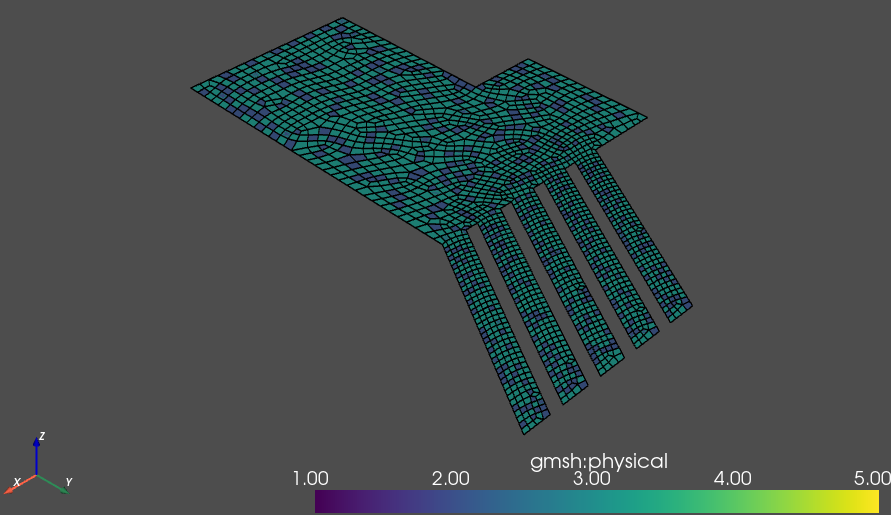
\includegraphics[width=\textwidth]{Images/CFDEM/malla.png}
	\caption{Mallado inicial de la geometr\'ia.}
	\label{malla:geo}
\end{figure}

\noindent
\justify

Se elabor\'o la malla con elementos rectangulares debido al mayor \'indice de precisi\'on en los resultados de simulaciones num\'ericas que emplean este tipo de elemento de malla$^{\cite{Tu2018, Illes2020}}$. Los elementos rectangulares presentan mayor facilidad de alcanzar la convergencia en t\'erminos de \textit{no ortogonalidad}$^{\cite{Tu2018, Martinez2019}}$ y a la baja \textit{oblicuidad}$^{\cite{Tu2018}}$. La malla mostrada en la Figura \ref{malla:geo} presenta las caracter\'isticas mostradas en el Cuadro \ref{malla}.

\begin{table}[h!]
	\centering
	\begin{tabular}{|c|c|}
		\hline
		\textbf{Par\'ametro} & \textbf{Valor} \\ \hline
		Tipo de elementos & Rectangulares \\ \hline
		N\'umero de elementos & 6097 \\ \hline
		N\'umero de nodos & 4560 \\ \hline
		Tama\~no m\'aximo de elementos $[\mu m]$ & $20000$ \\ \hline
		Tama\~no m\'inimo $[\mu m]$ & $10000$ \\ \hline	
	\end{tabular}
	\caption{Datos de la malla inicial generada.}
	\label{malla}
\end{table}

\newpage

\noindent
\justify

Al emplear el m\'etodo \texttt{checkMesh} de OpenFOAM para el an\'alisis preliminar de malla, se obtuvieron los siguientes resultados:

\begin{table}[h!]
	\centering
	\begin{tabular}{|c|c|}
		\hline
		\textbf{Par\'ametro} & \textbf{Valor} \\ \hline
		Apertura \textit{m\'axima} entre elementos & 21.20 \\ \hline
		Checkeo de \textit{no} ortogonalidad & OK \\ \hline
		Oblicuidad m\'axima & 0.78 OK \\ \hline
		Conclusi\'on de malla & OK \\ \hline
	\end{tabular}
	\caption{Resumen de resultados sobre el checkeo de malla.}
	\label{check}
\end{table}

\noindent
\justify

A partir de los resultados mostrados en el Cuadro \ref{check}, se concluye que la malla es apta para el desarrollo de las simulaciones num\'ericas consecutivas.